\documentclass[../main.tex]{subfiles}
\graphicspath{{\subfix{../figures/}}}

\begin{document}
\chapter{Controller Design} \label{chap:ctrl_design}
This chapter analyzes the core components of a Twin-Delayed Deep Deterministic (TD3) Policy Gradient agent and how I craft them. I also demonstrate best practices in fine-tuning hyperparameters and some significant experiments. 


\section{The Anatomy of TD3}
As I introduced in section \ref{sec:actor_critic}, TD3 is a \textbf{model-free, online} agent, so it does not store any snapshot of the environment but instead interacts directly. Again, our plant's dynamics are sluggish (Sec. \ref{sec:env_model}), so training on a practical system would take many days. To workaround this caveat, I will recreate the system, including the agent and the plant, in Simulink. On the other hand, TD3 is \textbf{off-policy, actor-critic-based}, so it requires a memory buffer to store past data for training, even when they do not come from the same policies. Since it is based on the actor-critic framework, to evaluate that action (Fig. \ref{fig:td3}). To overcome the overestimate of Q-value due to noises and quantization errors, TD3 uses:
\begin{enumerate}
    \item Learning two Q-value functions and using the minimum value function estimate during policy updates.
    \item Updating the policy and targets less frequently than the Q functions.
    \item When updating the policy, a TD3 agent adds noise to the target action, which makes the policy less likely to exploit actions with high Q-value estimates.
\end{enumerate}
\begin{figure}[htbp]
    \centering
    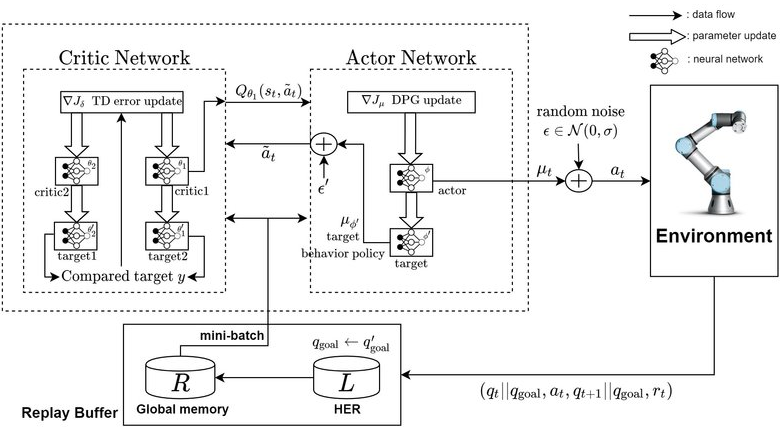
\includegraphics[width=\linewidth]{figures/td3.png}
    \caption{TD3 agent's components \cite{kim20motionplanning}}
    \label{fig:td3}
\end{figure}

One concern with deterministic policies is their tendency to overfit to narrow peaks in the value estimate. When updating the critic, using a deterministic policy as the learning target can be highly susceptible to inaccuracies induced by function approximation errors, leading to an increased variance in the target \cite{td3}. To mitigate this induced variance, the authors proposed a regularization technique called "target policy smoothing," which added a small amount of Gaussian noise $\epsilon$ to the target policy and averaged over mini-batches (Eq. \ref{eq:target_smoothing}).
\begin{align} \label{eq:target_smoothing}
    y &= r + \gamma Q_{\theta^\prime}(s^\prime, \pi_{\phi^\prime}(s^\prime) + \epsilon) \\
    \epsilon &\sim \text{clip} \left( \mathcal{N}(0, \sigma^2), -c, c \right)
\end{align}
We can choose the noise variance and boundary, but they suggested $\sigma = 0.2$ and $c = 0.5$, so I will keep them as is.

\section{Observation Space}
A continuous observation space $\mathbb{S}$ consists of real-value state vectors $\mathbf{s} \in \mathbb{S}:\mathbb{R}$ that provide valuable insights into our problem. Any missing information may prevent learnability. Let us not be confused $\mathbf{s}$ with the plant's state vector $\mathbf{x}$ in section \ref{sec:env_model}.
$$\mathbf{x} = \begin{bmatrix*}
    T_a \\
    T_f \\
\end{bmatrix*}$$
Sometimes, they can be equal, but in this case, $\mathbf{x}$ alone is not good enough. As I explain in section \ref{sec:rl_ctrl}, a vector $s \in \mathbb{S}$ can contain values from disturbances, filters, or actuator properties, as long as they are informative. To begin with, we must have the setpoint $T_{ref}$, controlled target $\overline{T}_a$, and floor temperature $T_f$ to make sure it never hits safety boundaries. Immediate room temperature $T_a$ and outside temperature $T_{out}$ should be known as well because they impact the system's dynamics, i.e., heat loss rate through walls (Sec. \ref{sec:env_model}). Theoretically, that is enough. 
$$\mathbf{s} = \begin{bmatrix*}
    T_{ref} \\
    T_f \\
    T_a \\
    \overline{T}_a \\
    T_{out} \\
\end{bmatrix*}$$

 Nevertheless, augmentation is still necessary to gain better performance. Firstly, $T_{ref}$ is useless to a neural network because it is constant. Indeed, any low-variance feature provides no helpful information. A better way to encapsulate this is using the error $e = T_{ref} - T_a$. This feature notifies how far it is from the target. Yet, picking the right $T_a$ is challenging as it is returned from sensors every millisecond. However, observing the state change takes a few minutes. Thus, utilizing the average temperature between two timestamps when the agent makes decisions is sensible.
    $$
    \overline{T}_a \defeq \frac{1}{\tau_s}\int_{t}^{t+\tau_s} T_a \,dt
    $$
\begin{itemize}
    \item $\tau_s$: agent's sampling time
\end{itemize}
$T_f$, on the other hand, should continue to be recorded in real-time due to its safety-critical function. Similarly, I choose the difference between inside and outside temperatures $\Delta T = T_a - T_{out}$ instead of $T_{out}$. This feature directly implies how rapid and in which direction the heat transfer occurs. Another common practice is using the error integral to reduce steady-state error and yield faster convergence \cite{weber2022ss}. 

Given that the outside temperature $T_{out}(k)$ can be predicted for any given timestamp $k$ through weather forecasting, utilizing its projected value $T_{out}(k+1)$ could facilitate disturbance rejection. While such a strategy is effective in model-based algorithms like MPC, its usage in TD3 is not feasible because our agent must consider the future state $\textbf{x}(k+1)$, which remains unknown due to its lack of insight into the plant's dynamics. Some researchers have worked on this matter, but they all end up being model-based \cite{chen2019gnu,fu21mpctd3}.

The adaptability of the conduction coil's load $I \,(A)$ to accommodate various house sizes enhances its utility. For instance, larger homes need a greater load to expedite heating. As a result, incorporating this variable can bolster the resilience of TD3 against fluctuations in load during practical tests.

In their theses, Junior \cite{junior22} and Sebastian \cite{seb23} added the last action to the observation space. I argued that this is not a good practice as it breaks Markov's property, i.e., the future state must only depend on the current state and action, not on the history of past states and actions. Such violated setups are called non-Markovian decision processes that are unsuitable for traditional RL. In summary, my final observation vector is

\begin{equation}
    \mathbf{s} = \begin{bmatrix*}
        T_f \\
        T_a \\
        T_{ref} - \overline{T}_a \\
        \int_{0}^{t} (T_{ref} - T_a) \,dt \\
        T_a - T_{out} \\
        I
    \end{bmatrix*}
\label{eq:obs}
\end{equation}

\section{Action Space} \label{sec:agent_action}
\subsection{Agent's Sampling Time and PWM Period}
Since UWG5's PWM period varies between 10 to 20 minutes (\ref{sec:env_baseline}), it is disadvantageous for debugging and predictive maintenance. Even worse, figure \ref{fig:actual_dynamics} shows that this strategy usually operates at 10 minutes; it rarely extends any longer. Empirically, we limit our experiments to 12 and 15 minutes to balance predictability and device longevity. Other trials showed that 18 and 20 minutes are unstable and often yield greater overshooting. 
    $$P \in \{ 0.2, 0.25 \} \text{ (hours)}$$

On the other hand, an agent's sampling time $\tau_s$ is tightly dependent on the actuator's properties. Commonly, RL agents require instant feedback to avoid the sparse reward problem (Sec. \ref{sec:rwdfcn}) or mismatching feedback from other actions. Thus, its sampling time must be no less than the actuation time.
    $$\tau_s \geq P$$
Starting with $\tau_s = P = 0.2$ (hours) and a vanilla reward function (Sec. \ref{sec:rwdfcn}), the agent successfully brings the immediate air temperature $T_a$ into the maximum-reward zone $\pm 1$ (\degree C) at every timestamp $\tau_s$. However, an overshot $T_a$ can still repeat during this interval, hence a non-zero steady-state error of $\overline{T}_a$ (Fig. \ref{fig:sse}).
\begin{figure}[htbp]
    \centering
    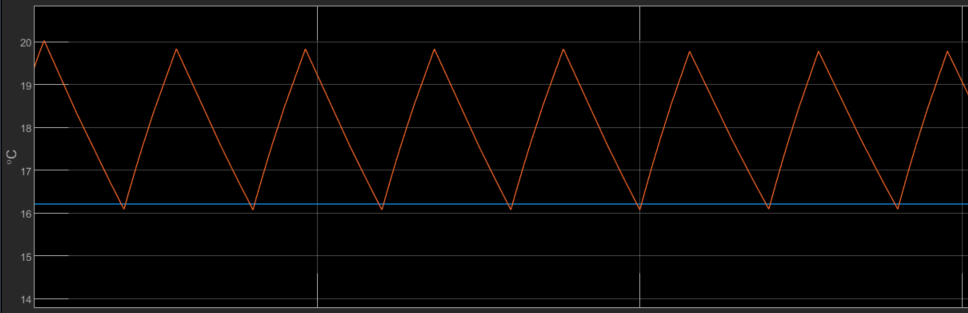
\includegraphics[width=1\linewidth]{figures/false_positive_policy_result.png}
    \caption{Steady-state error of the average air temperature}
    \label{fig:sse}
\end{figure}
Indeed, such a periodic phenomenon occurs for all $\tau_s = nP$ where $n \in \mathbb{N}^*$. So I chose $\tau_s \neq P$ in the second experiment
\begin{equation}
    \begin{cases}
        P = 0.2 \,(\text{hours}) \\
        \tau_s = 0.25 \,(\text{hours})
    \end{cases}
\end{equation}
Then, the relay is turned on twice per sampling interval, and the agent retrieves an observation during the heating phase. Thus, the temperature peak should not exceed our setpoint to gain more reward, hence a smaller steady-state error (Fig. \ref{fig:choose_p_ts}.
\begin{figure}[htbp]
    \centering
    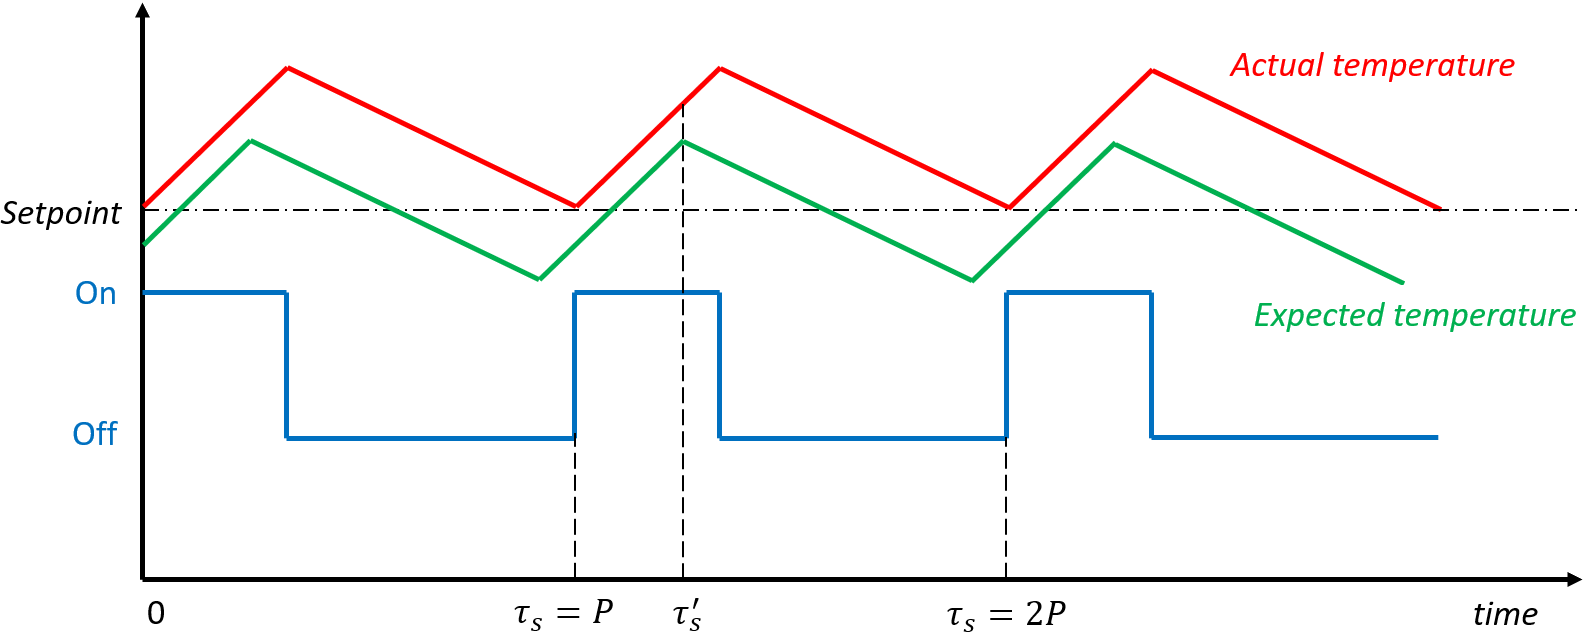
\includegraphics[width=1\linewidth]{figures/choosing_P_Ts.png}
    \caption{How to choose $T_s$ accordingly to $P$}
    \label{fig:choose_p_ts}
\end{figure}


\subsection{Action Data Type}
Theoretically, that action is fine. Yet, implementing it under a proper data type is non-trivial in real software development since it affects our training process. Specifically, MATLAB declares an agent's action $a = D$ as a 64-bit float ($\mathtt{double}$)\textemdash a gigantic exploration space. Meanwhile, UWG5's predefined interface only accepts a 16-bit float (half precision) and actuates with four decimals, e.g., $D = 0.1234$ (\%). Consequently, leaving that default data type for training wastes time and is meaningless. Sometimes, it might not even work when combined with a suboptimal reward function (Fig. \ref{fig:double_action}). 
\begin{figure}[htbp]
    \centering
    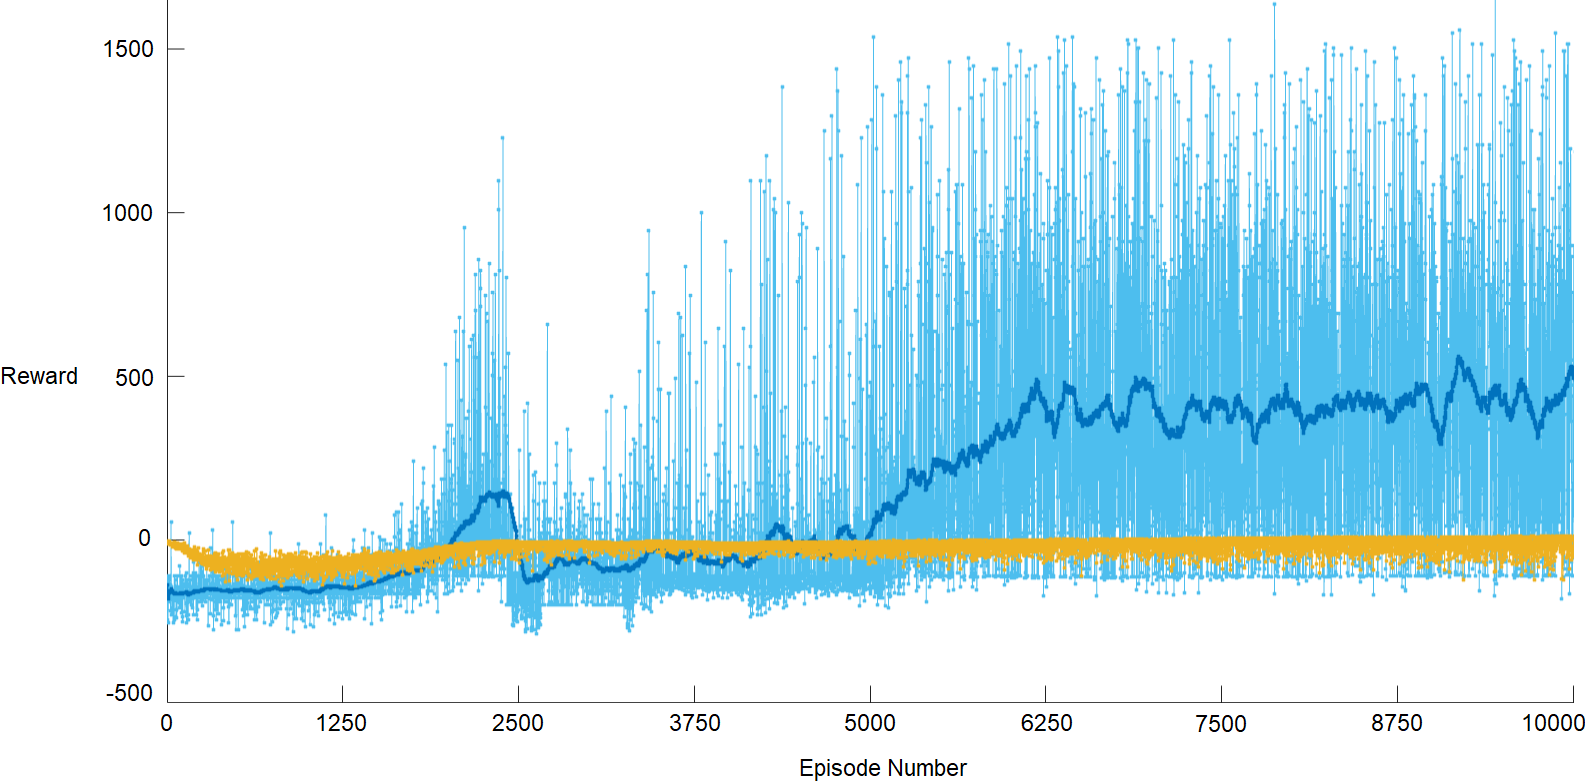
\includegraphics[width=1\linewidth]{figures/double_action.png}
    \caption{$\mathtt{double}$ action space has long convergence time}
    \label{fig:double_action}
\end{figure}
So, I assign it to an 8-bit unsigned integer, turning the action space into a finite set of only 100 possibilities. An action is then converted into PWM by dividing 100 (Eq. \ref{eq:uint8_action}). Figure \ref{fig:training_result} in section \ref{sec:train_val} confirms my idea.
\begin{equation}
\begin{split}
    a \in \mathbf{A} &= \mathbb{N} \rightarrow \mathtt{uint8} \\
    D &= a/100
\end{split}
\label{eq:uint8_action}
\end{equation}

\textbf{An important note} for reading the training results of an RL agent using MATLAB Reinforcement Learning Toolbox, such as figure \ref{fig:double_action} or \ref{fig:bar_rwd}:
\begin{itemize}
    \item \textbf{Dark blue line} represents the average reward of the latest 100 episodes, which infers the actor's learning status.
    \item \textbf{Light blue dots} are the instantaneous reward per episode.
    \item \textbf{Orange line} represents the expected reward of the current episode using the last policy, which infers the critic's learning status.
    \item Generally, the blue line is more important. A successful session should have an upward trend followed by saturation. The orange line, in fact, is not as important. It can either incline or decline before saturating. The actor (blue line) may converge first and it is fine to stop training \cite{matlab_q0_support}.
\end{itemize}

\section{Agent} \label{sec:agent}
The above state and action definitions decide an agent's input and output layers. Now, I only have to tune the hidden layers.

\subsection{Actor's Network}
Based on my experience with deep learning, I assigned the actor two 256-node dense layers with ReLU activation. Since the output is continuous between zero and one, I endorse a $\tanh$ activation in the single-node output layer. Such a setup is complex enough to avoid overfitting without compromising approximation capability (Fig. \ref{fig:actor}).
\begin{figure}[htbp]
    \centering
    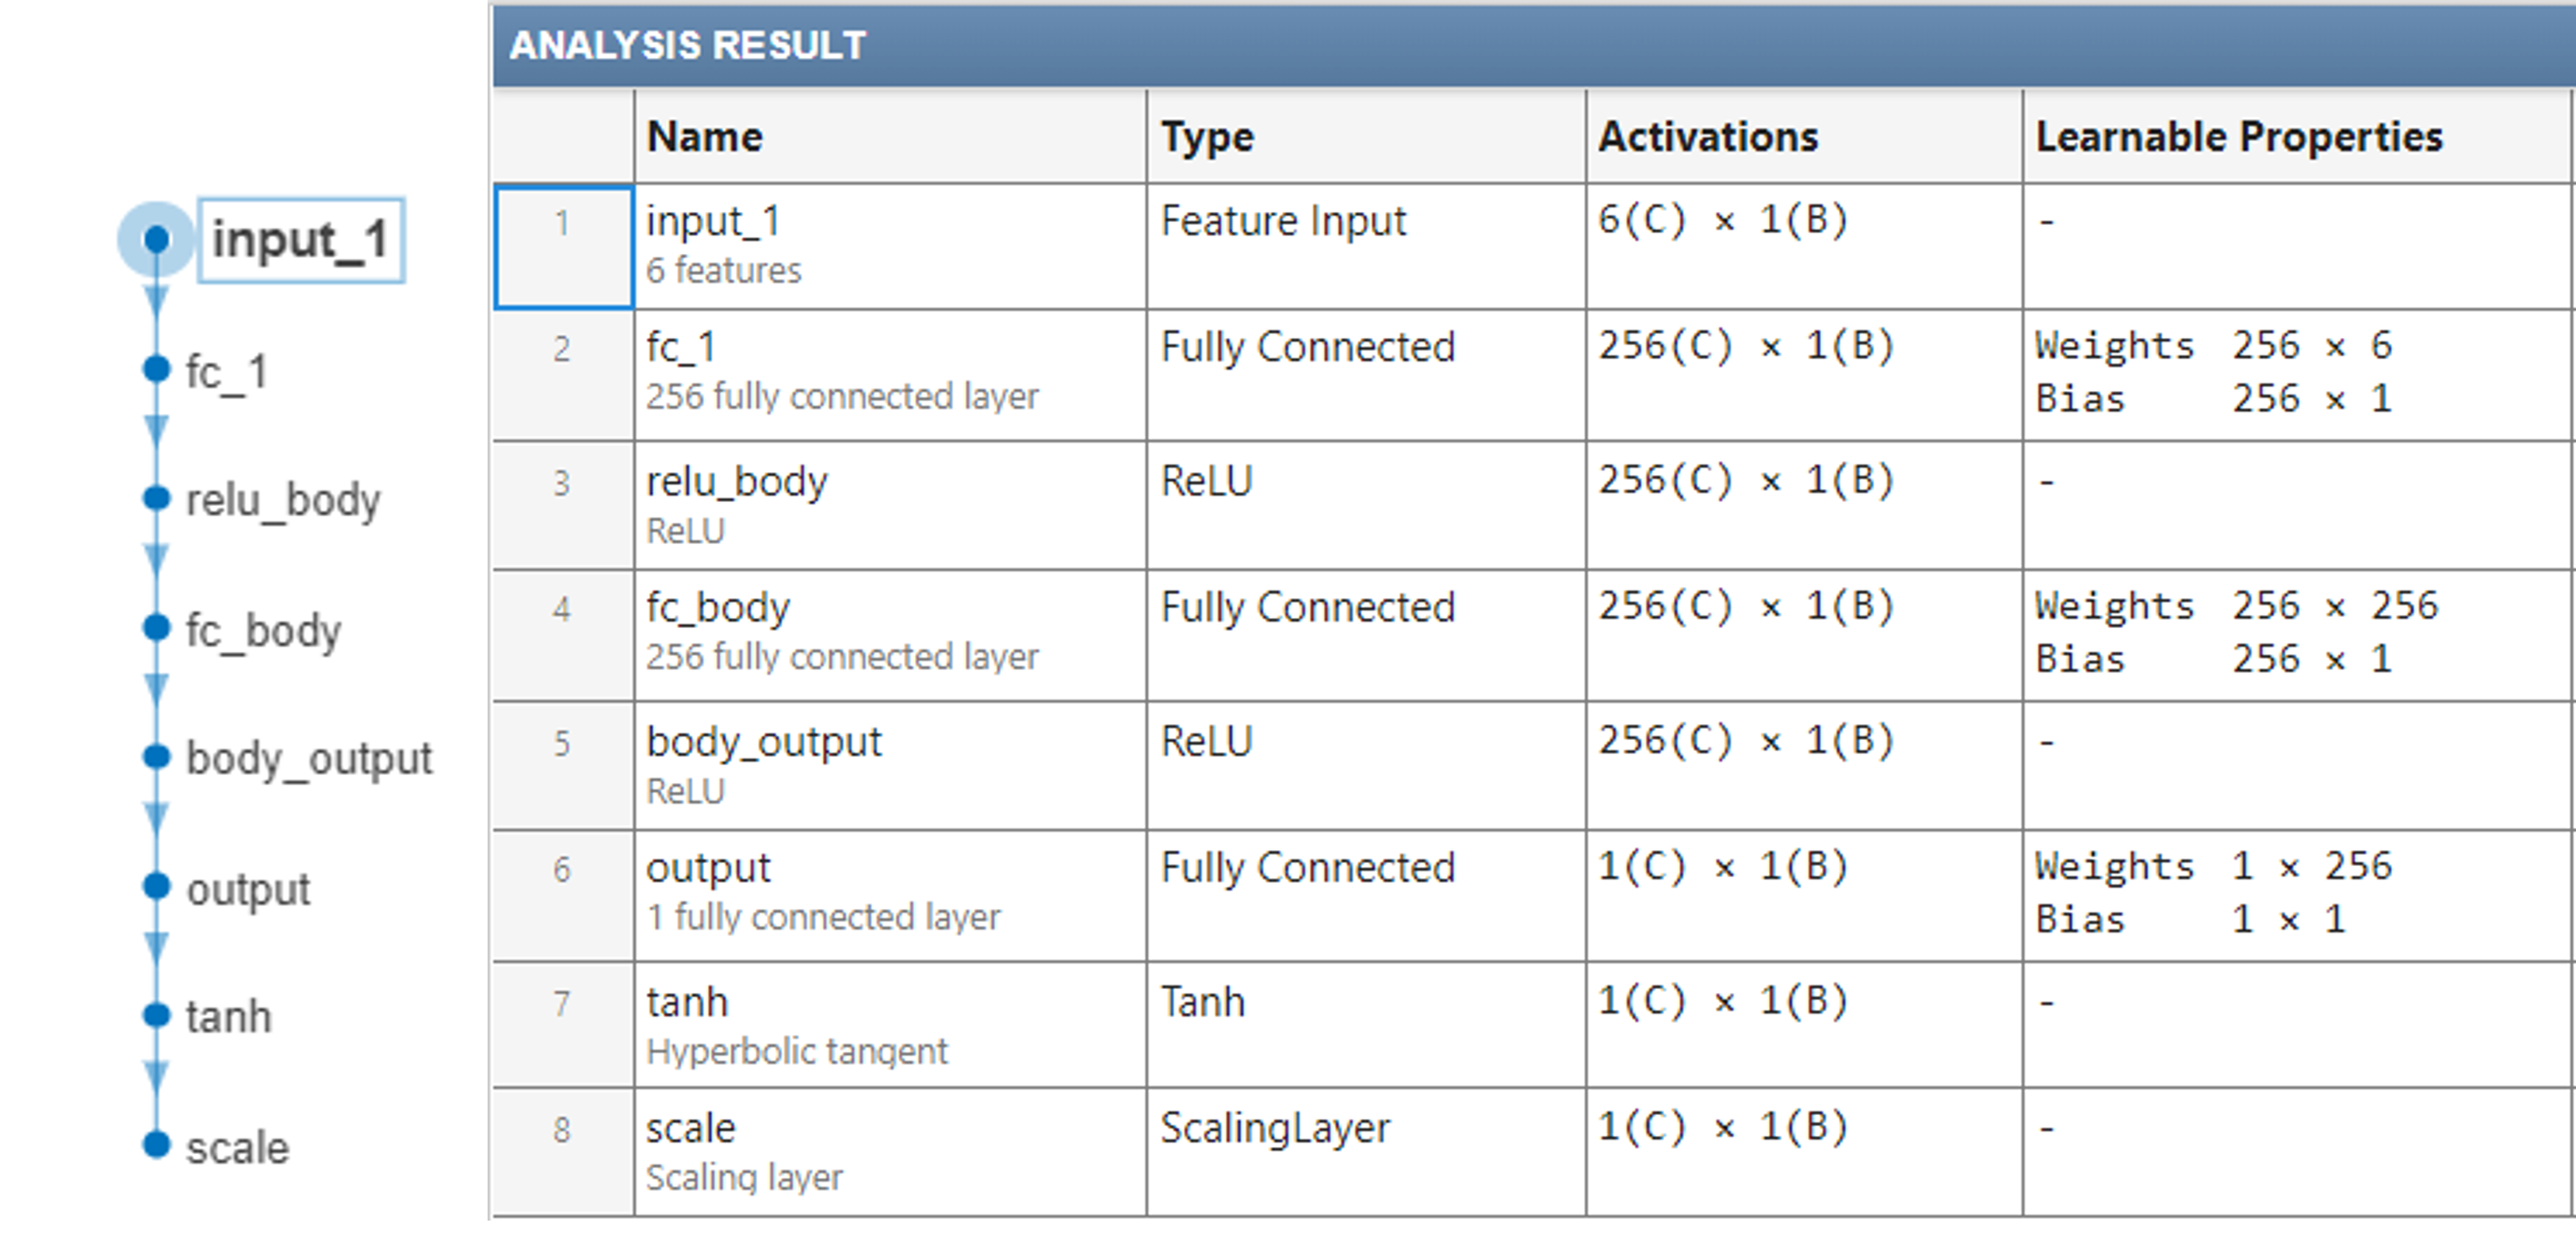
\includegraphics[width=1\linewidth]{figures/actor_network.png}
    \caption{Architecture of TD3's actor}
    \label{fig:actor}
\end{figure}

\subsection{Critic's Network}
Designing a critic is a bit more complex since its input consists of two paths: observation, a 6-element vector, and action, a scalar. Two dense layers transform each of them linearly before returning their concatenation as a scalar Q-value. I also default 256-node dense layers (Fig. \ref{fig:critic}).
\begin{figure}[htbp]
    \centering
    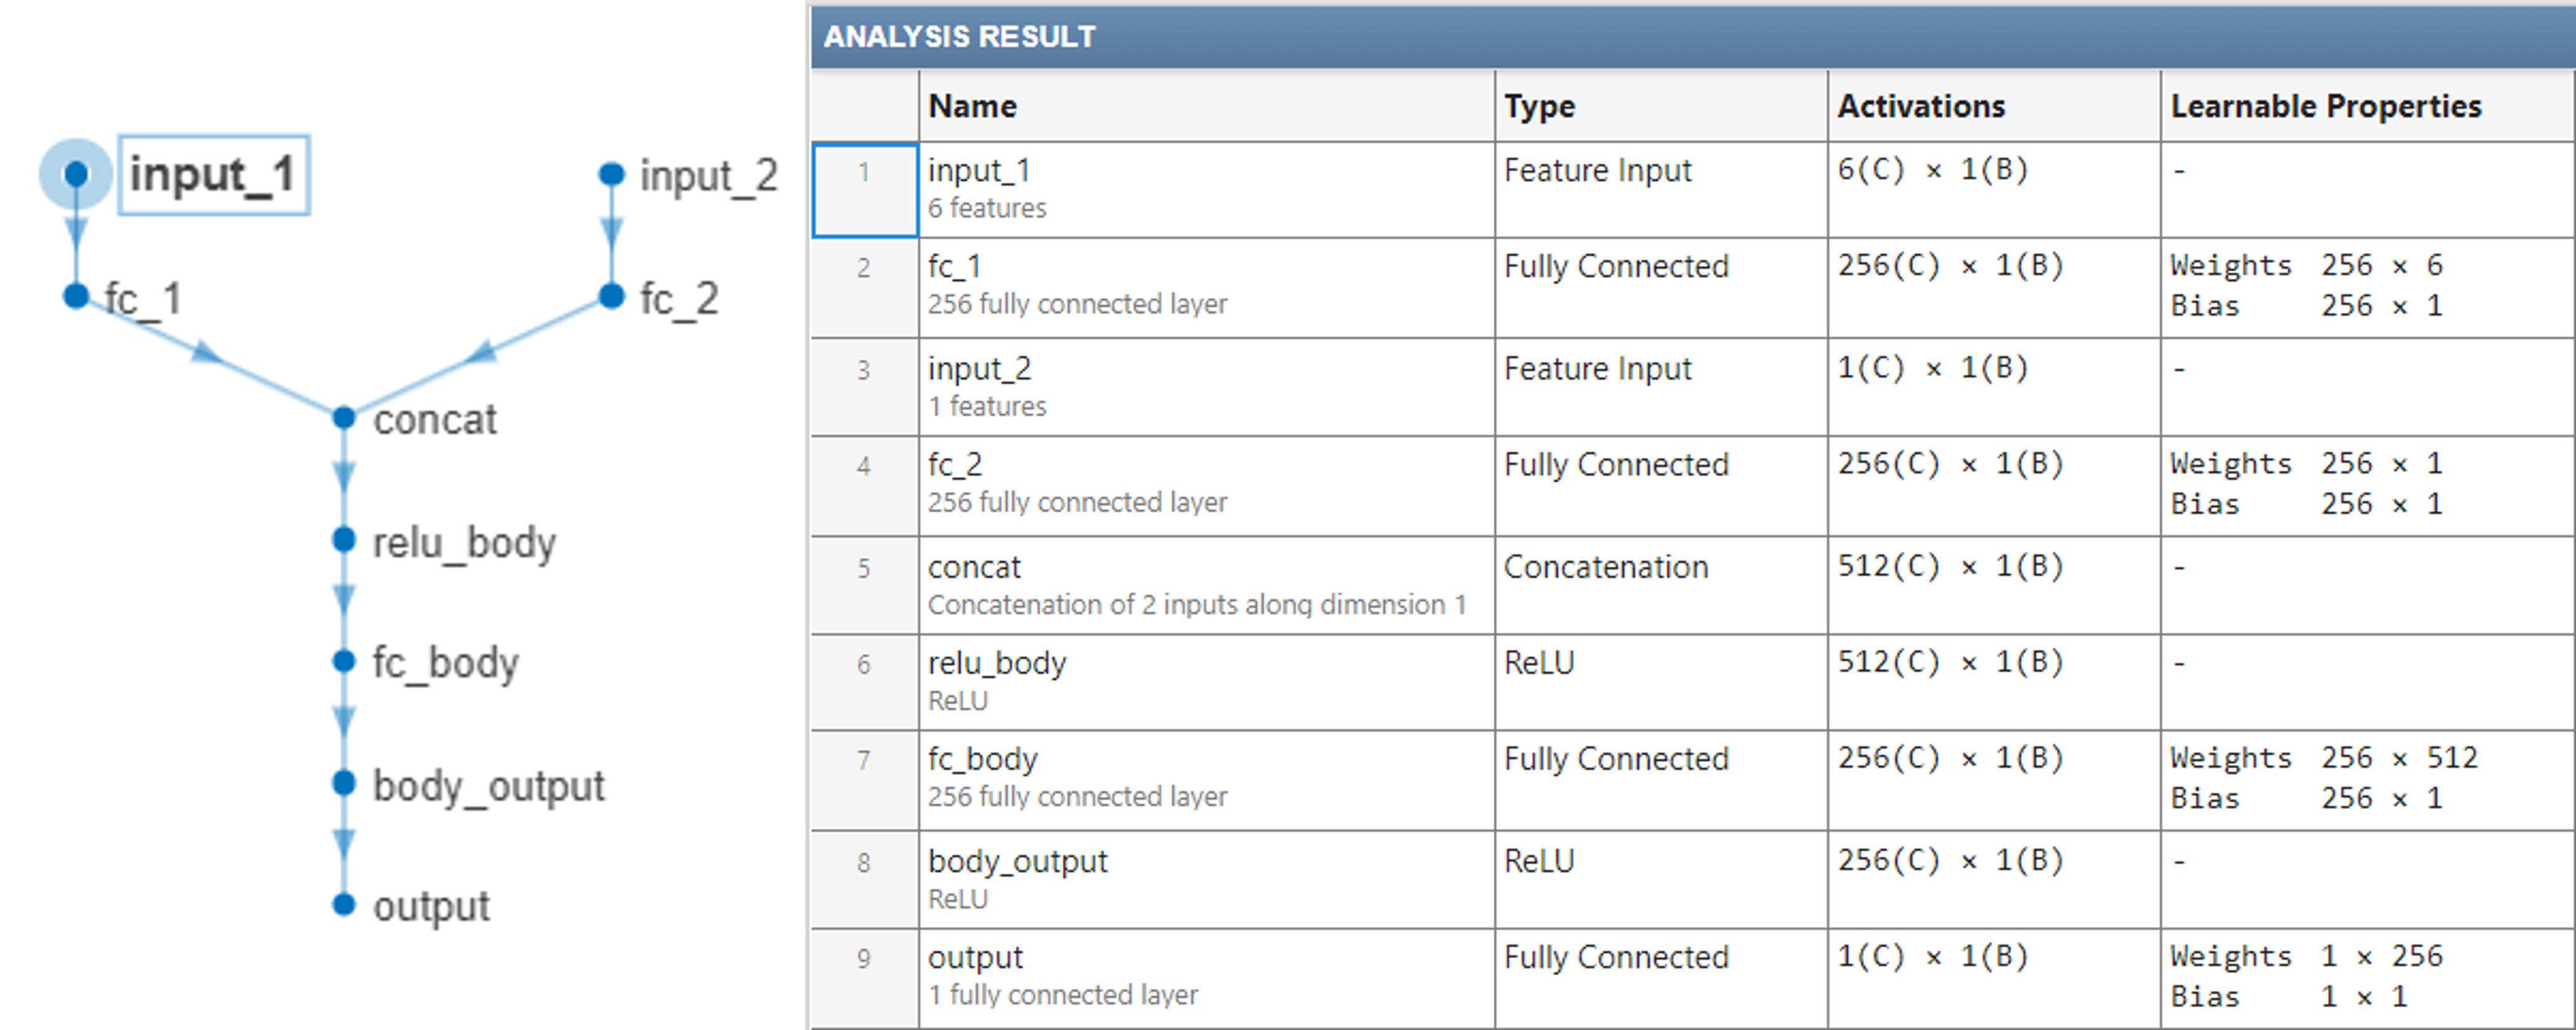
\includegraphics[width=1\linewidth]{figures/critic_network.png}
    \caption{Architecture of TD3's critic}
    \label{fig:critic}
\end{figure}

Again, the above parameters were chosen based on my fuzzy experience from my "Advanced Machine Learning" course at SDU and some trial and error. Further tuning with automation tools such as Python's Optuna exceeds our computational resources and is beyond this thesis' scope.


\section{Reward Function} \label{sec:rwdfcn}
In RL, a reward function is fundamental in guiding an agent's behavior towards achieving its goals. The reward function $R_t = R(s_t,a_t,s^{\prime}_t)$ defines the immediate feedback the agent receives upon taking action $a_t$ to transition from its current state $s_t$ to the next one $s^{\prime}_t = s_{t+1}$. This formulation quantifies state-action desirability, indicating how favorable or unfavorable they are towards the agent's objective. A well-designed reward function makes faster training and better control performance. Depending on the nature of the problem, a reward function can be discrete, continuous, or both. This subsection presents some candidates of those types.

\subsection{Discrete Reward}
A discrete reward function exhibits discontinuous variations in response to state-action changes. Typically, these reward functions are triggered by individual events within the environment. For instance, an agent might receive a positive reward only when it reaches a predefined target. To illustrate this concept, consider a straightforward formulation: let the agent attempt and give it a 10-point bonus if it gets close to the setpoint, i.e., a tolerance of $\pm 1$ (\degree C) and 0 points otherwise.
\begin{equation}
    R_t = \left\{ \begin{aligned}
        10 & \text{ if $\abs{e_t} \le 1$} \\
         0 & \text{ if $\abs{e_t} > 1$}
    \end{aligned}\right.
\end{equation}
This might work for a finite state-action space like a maze-solving game, despite excessive exploration steps \cite{hare2019dealing}. However, when I tried, it was disastrous (Fig. \ref{fig:sparse_rwd}). The problem is known as a "sparse-reward environment," which confuses the agent by not giving sufficient feedback. A resolution requires reward engineering techniques such as "reward shaping" \cite{Ng1999PolicyIU, miller2023rewardshaping} or "Q-value initialization" \cite{eric03rwd}. 
\begin{figure}[htbp]
    \centering
    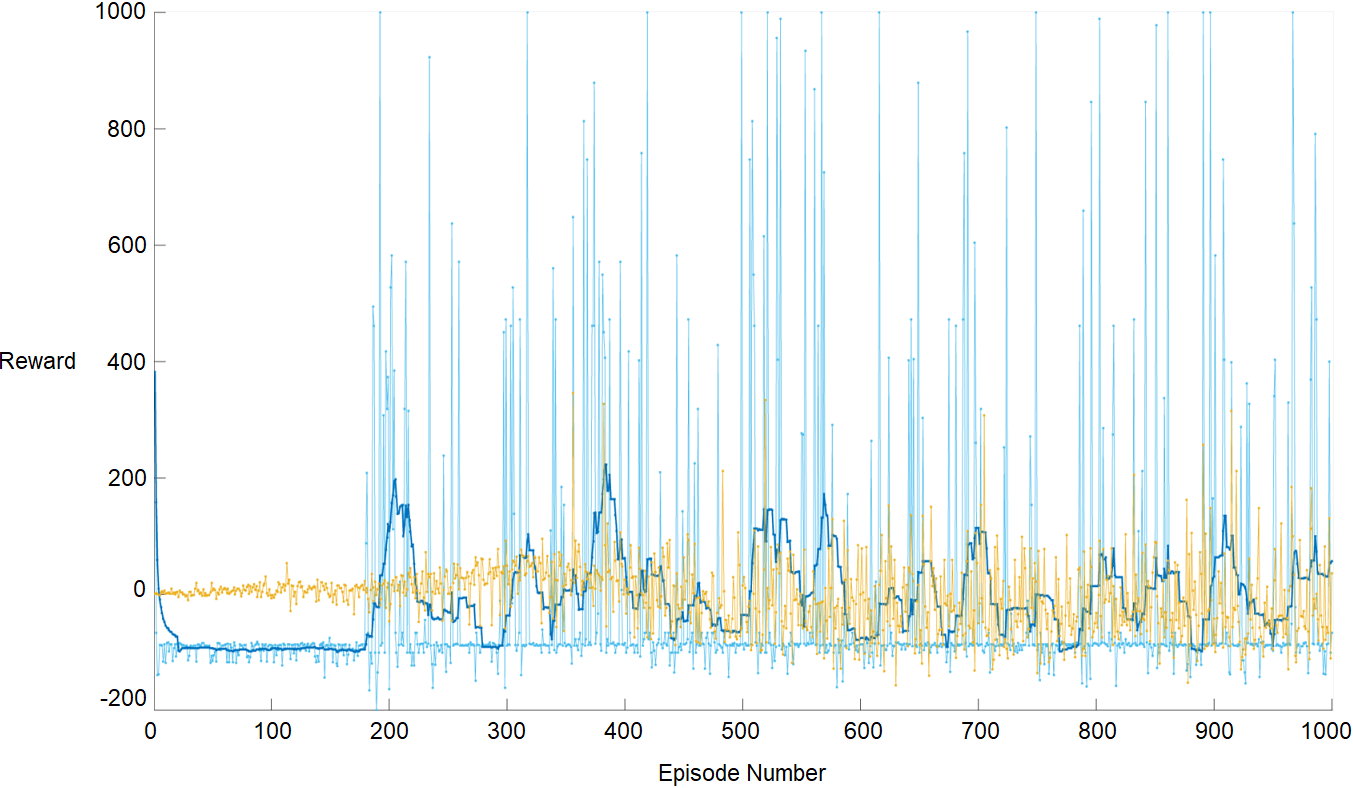
\includegraphics[width=1\linewidth]{figures/sparse_rwd.png}
    \caption{Sparse reward problem}
    \label{fig:sparse_rwd}
\end{figure}

Before putting on any of these fancy clothes, I try a tiny change first: instead of giving nothing, now we provide a minus if the agent does not reach the target as a notion of "bad choice"(\ref{eq:vanilla_rwd}). 
\begin{equation} \label{eq:vanilla_rwd}
    R_t = \left\{ \begin{aligned}
        10 & \text{ if $\abs{e_t} \le 1$} \\
        -1 & \text{ if $\abs{e_t} > 1$}
    \end{aligned}\right.
\end{equation}
As a result, the agent now knows which action to avoid in the future if it gets the same observation $s$ again. I call this \textbf{a vanilla reward function}. Although it works well, training is so slow (Fig. \ref{fig:vanilla_rwd}) that there are 1,600 episodes before convergence. Furthermore, such a discrete function often requires more complex network structures because it only tells whether an action is good or bad, but not how much \cite{MathWorksReward2021, rlbible_rewarddesign}. That said, they can still guide the agent toward better locations in the environment's state space. For example, a region-based reward, such as a fixed reward when the agent is near a target location, can emulate final-state constraints. Also, a region-based penalty can encourage an agent to avoid certain areas of the state space.
\begin{figure}[htbp]
    \centering
    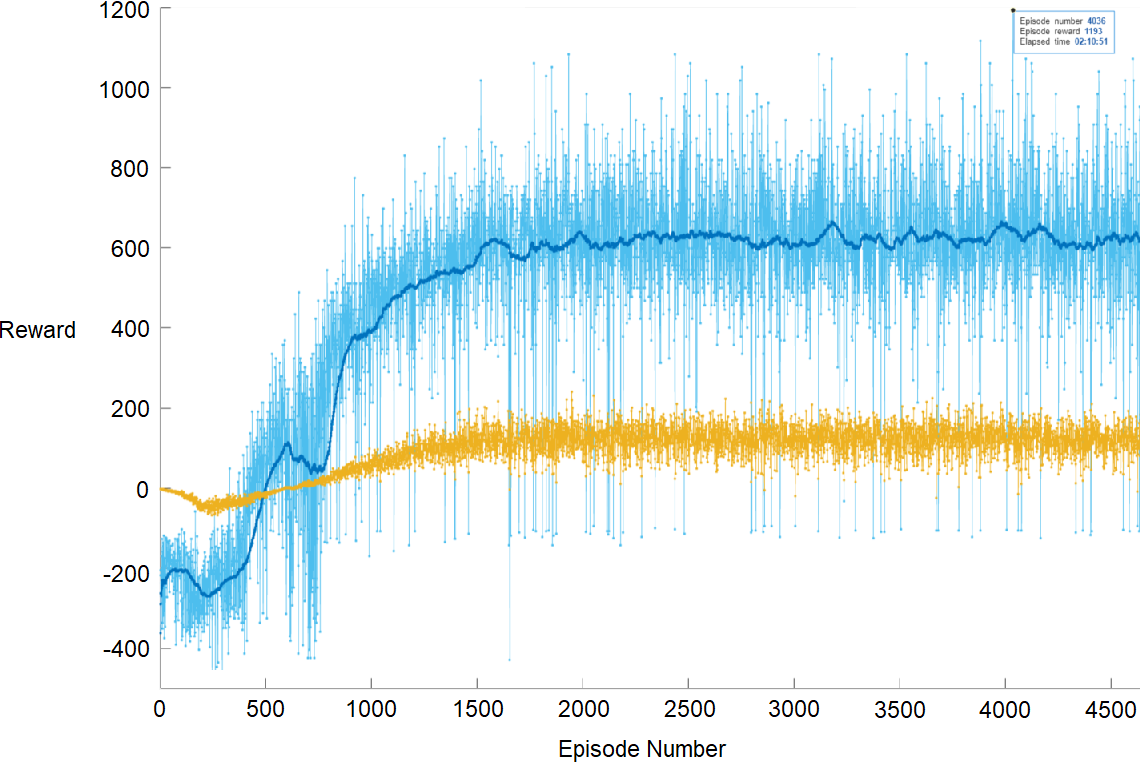
\includegraphics[width=1\linewidth]{figures/vanilla_rwd.png}
    \caption{Vanilla reward helps}
    \label{fig:vanilla_rwd}
\end{figure}

\subsection{Continuous Barriered Reward}
A continuous reward function varies continuously with environmental changes, observations, and actions. In general, continuous signals improve convergence during training and can lead to simpler network structures \cite{MathWorksReward2021, rlbible_rewarddesign}. Due to the continuous nature of our problem, in both observation and action, a smooth reward might yield a more refined definition for the state-action value. In other words, the agent receives an increasing reward as it gets closer to the target or a penalty otherwise. An effective candidate is the so-called \textbf{exponential barrier function} (Fig. \ref{fig:barrier_fns}) recently proposed by Nilaksh et al. \cite{nilaksh2024barrier}. They claimed that these functions not only make training faster but also enhance safety barriers.
\begin{align}
    h_{quad}(s_i, s_o) &= \sum_{l \in C} a_l \left( s_{il}^{max} - s_i \right) \left( s_i - s_{il}^{min} \right) 
    \label{eq:quad_barrier} \\
    h_{exp}(s_i, s_o) &= \sum_{l \in C} a_l \left( 1 - e{-\phi_lb(s_{il}^{max}-s_i)} + e{-\phi_lb(s_i-s_{il}^{min})} \right)
    \label{eq:exp_barrier}
\end{align}
\begin{figure}[htbp]
    \centering
    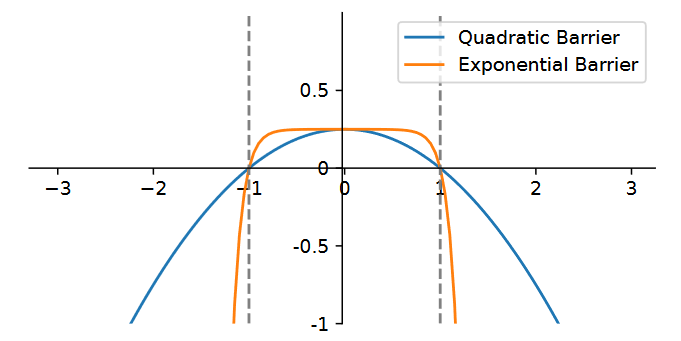
\includegraphics[width=0.75\linewidth]{figures/barrier_fns.png}
    \caption{Barrier functions. Dashed lines are the limits}
    \label{fig:barrier_fns}
\end{figure}

However, my experiments show that my agent could not find any positive solution under these proposals (Fig. \ref{fig:bar_rwd}). Despite an upward trend followed by saturation, the total rewards never rise above zero, i.e., output $T_a$ never stabilizes around our target. It is evident that heavy punishment is not encouraged for slow dynamics systems because the agent might not understand why a good action (e.g., moving toward the goal) still gives a big minus.
\begin{figure}[htbp]
\centering
\begin{subfigure}{\textwidth}
    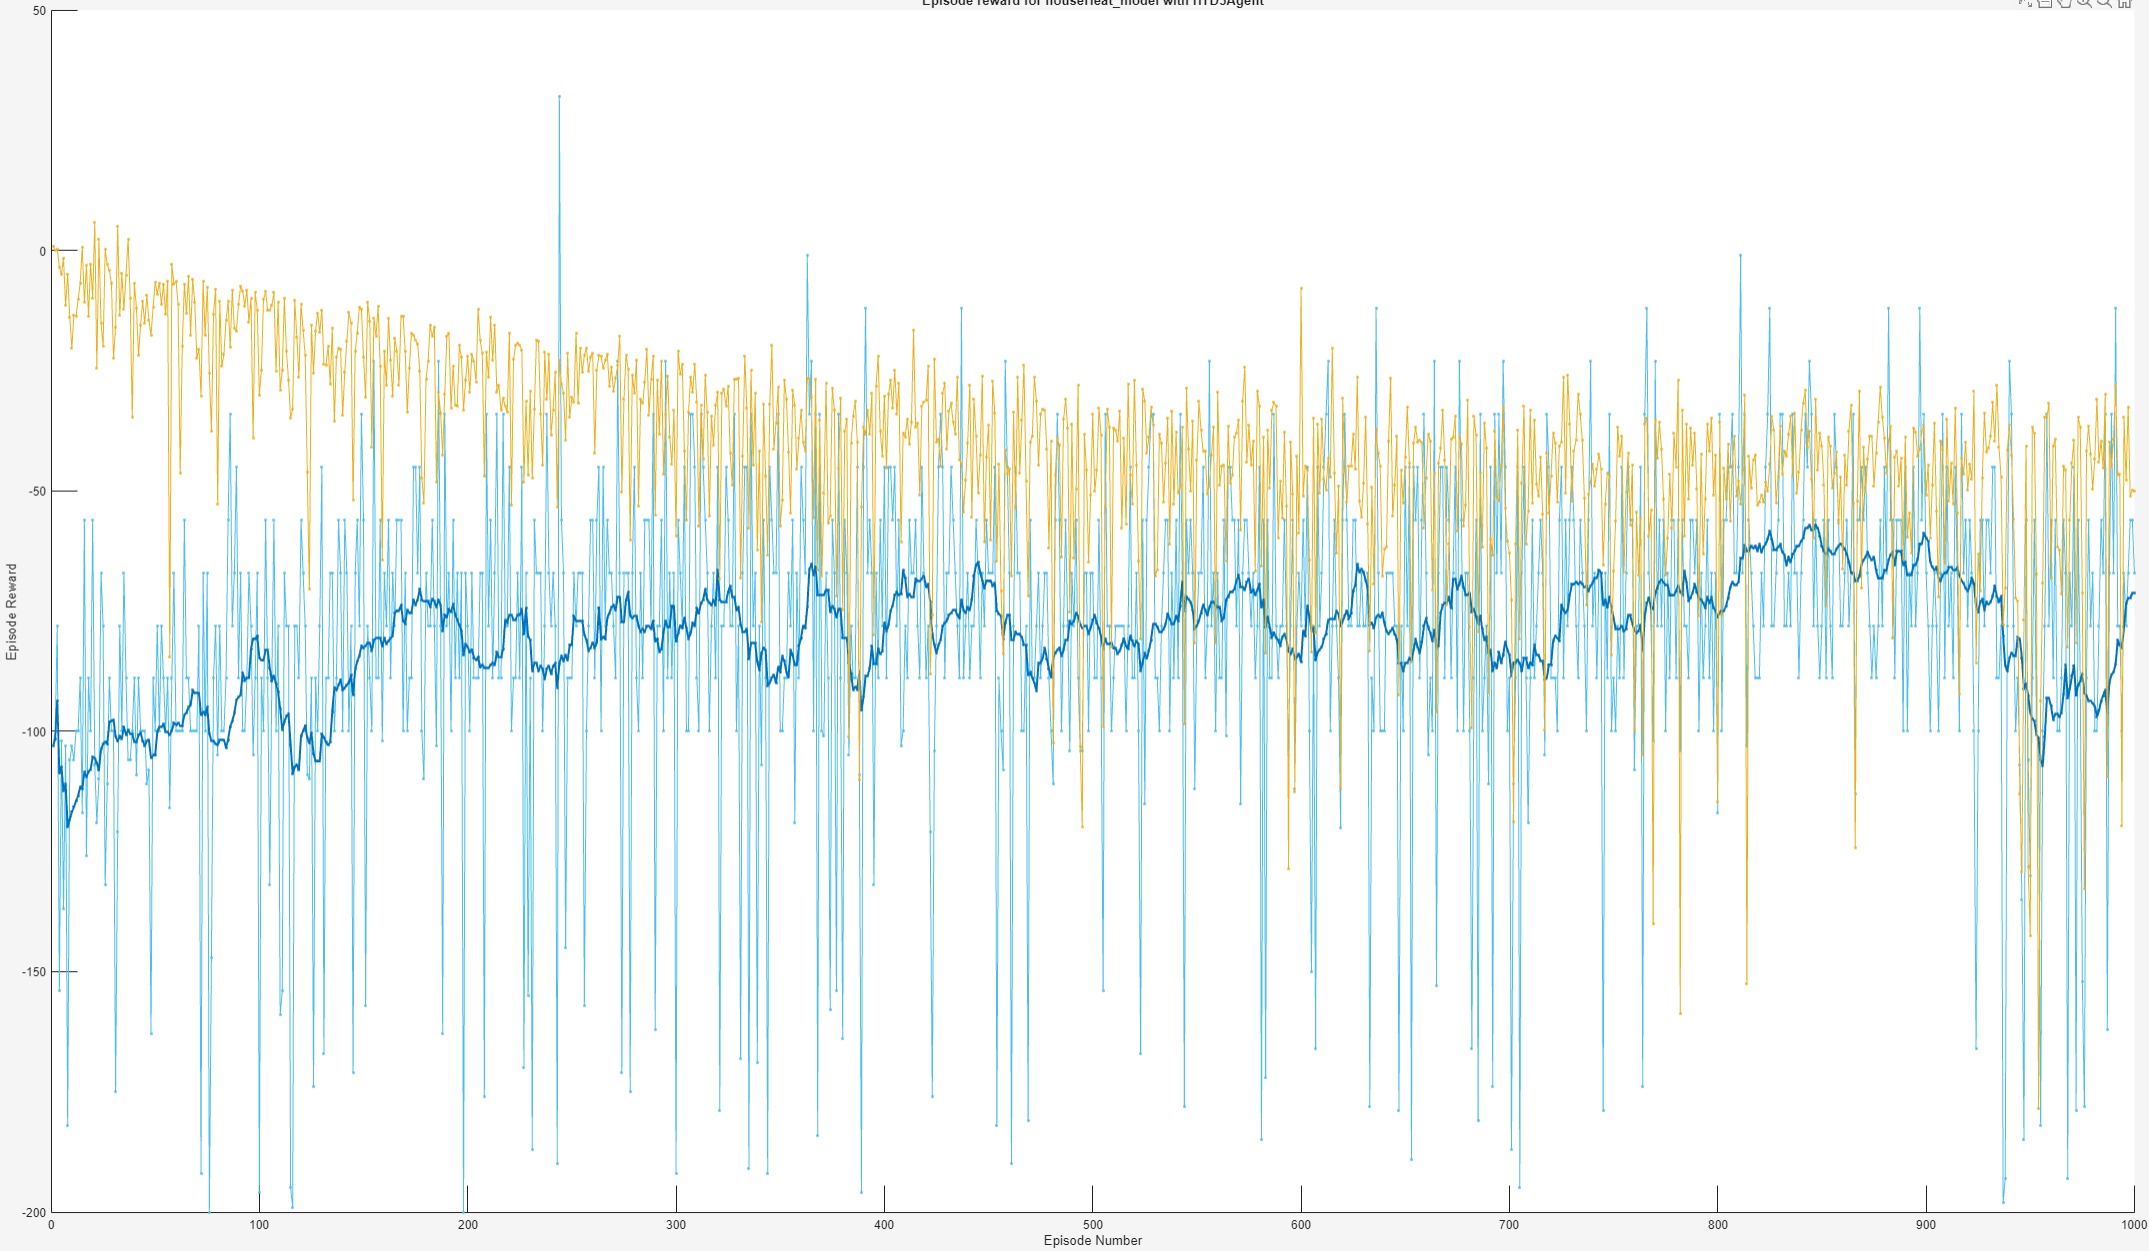
\includegraphics[width=\linewidth]{figures/quadbar_rwd.png}
    \caption{Training result with quadratic barriered reward}
    \label{fig:quadbar_rwd}
\end{subfigure}
\begin{subfigure}{\textwidth}
    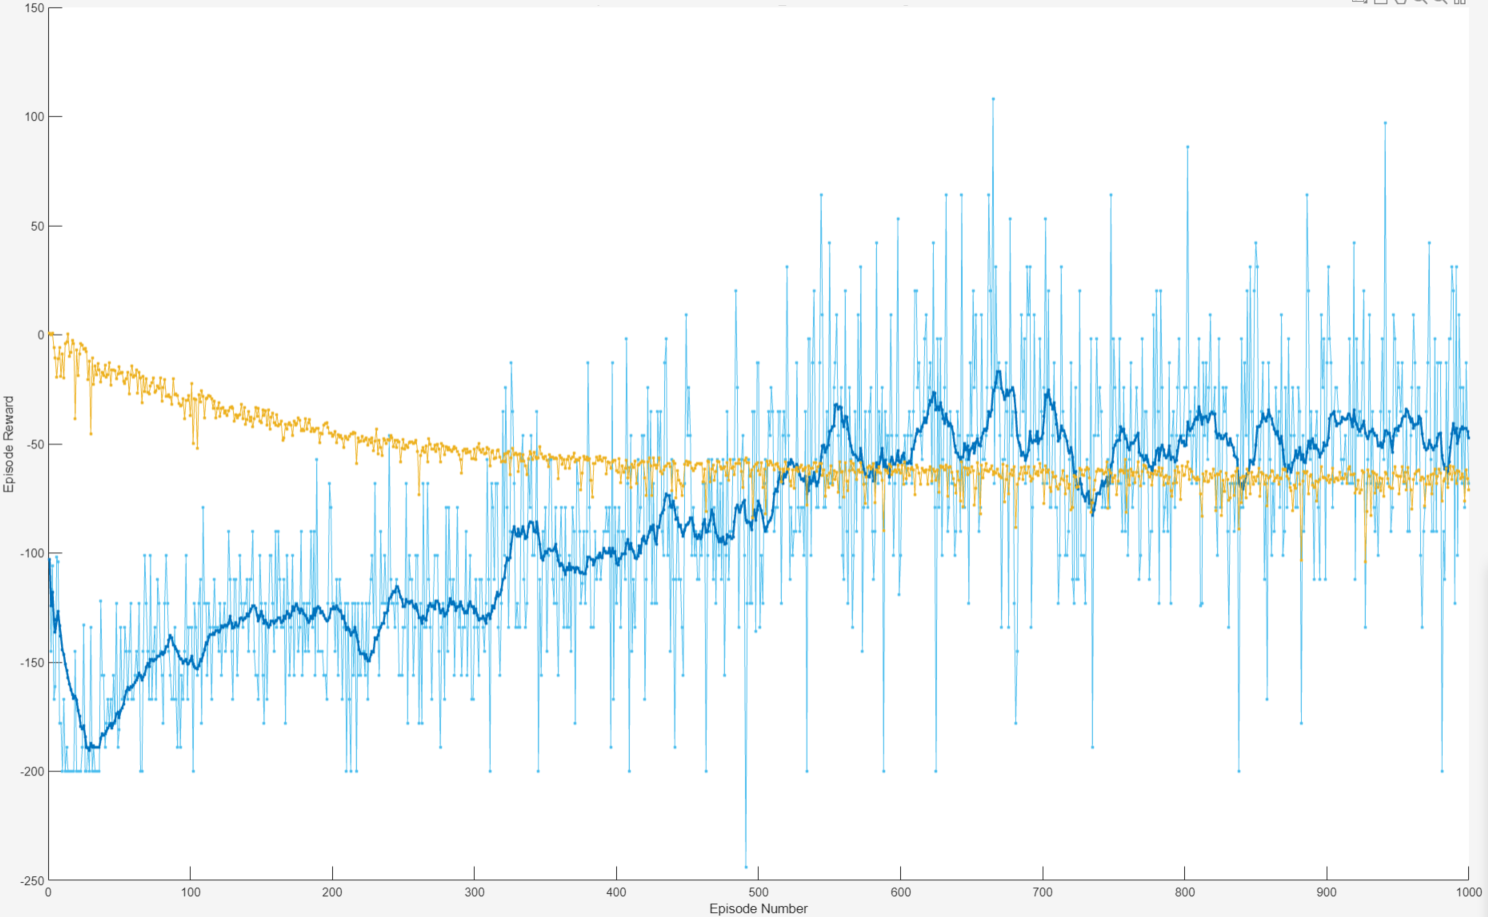
\includegraphics[width=\linewidth]{figures/expbar_rwd.png}
    \caption{Training result with exponential barriered reward}
    \label{fig:expbar_rwd}
\end{subfigure}
\caption{Training results with barriered reward functions}
\label{fig:bar_rwd}
\end{figure}

\subsection{Linear Quadratic Reward}
Another continuous formula is a linear quadratic (LQ) reward function (Eq. \ref{eq:lqrwd}), which creates a policy that is similar to classical optimal controllers (e.g., model predictive control) \cite{zhou2022single, matlab_obsrwd}.
\begin{equation}
    R_t = - \left( \mathbf{s}_t^\top \mathbf{Q} \mathbf{s}_t + \mathbf{a}_t^\top \mathbf{R} \mathbf{a}_t + 2\mathbf{s}_t^\top \mathbf{N} \mathbf{a}_t \right)
\label{eq:lqrwd}
\end{equation}
\begin{itemize}
    \item $\mathbf{Q}$ tunable weight matrix of states
    \item $\mathbf{R}$ tunable weight matrix of actions
    \item $\mathbf{N}$ tunable joined weight matrix of state-action
\end{itemize}
This formula is prevalent among control tasks. Yet, the naive form \ref{eq:lqrwd} focuses on bringing all states to zero and minimizing acting efforts. In contrast, we only aim at driving the average air temperature $\overline{T}_a$ to setpoints with minor priority in saving energy, so I modify it (Eq. \ref{eq:my_lqrwd}) with only error $e$ and PWM duty cycle $D$. Weights are freely tuned, starting with Bryson's rule, as long as $Q > R$.
\begin{equation}
    \begin{split}
        R_t &= - \left( Qe^2 + Ra^2 \right) \\
          &= - \left( 0.04(T_{ref} - \overline{T}_a)^2 + 0.01D^2 \right)
    \end{split}
\label{eq:my_lqrwd}
\end{equation}

\subsection{Terminal State Reward}
A terminal state is the final state of a training episode, which returns a terminal-state reward. It occurs when our agent reaches the maximum number of steps or hits the safety boundary. Typically, we do not need to give any reward in the first case, but we need a severe punishment in the latter case to remind them: "Don't do it again!"
\begin{equation} \label{eq:termrwd}
    R = \left\{ \begin{aligned}
        0 & \text{ when finishes} \\
        -100 & \text{ when violates safety boundaries}
    \end{aligned} \right.
\end{equation}

The bound is from 5 (\degree C) (to avoid being frozen) to 40 (\degree C) (to avoid cracking) for concrete. It is critical that in the MATLAB implementation, the feedback cycle of $T_f$ must be much faster than the agent’s sampling time $\tau_s$. This ensures that we never exceed safety limits. Otherwise, $T_f$ might still violate these limits during a sampling interval and drop back into the safe zone without the agent knowing.

\subsection{Hybrid Reward}
Naturally, we can mix those reward types to make use of their benefits, i.e., a discrete reward signal can be used to drive the system away from bad states, a continuous reward signal can improve convergence by providing a smooth trajectory toward targets, and a terminal penalty signify lethal behaviors. Afterward, I end up using
\begin{equation}
    R_t = \left\{ \begin{aligned}
        &+10 \text{  if } \abs{e} \leq 1 \\
        &-100 \text{  if } T_f \notin [5,40] \\
        &- \left[ 0.04(T_{ref} - \overline{T}_a)^2 + 0.01D^2 \right] \text{  any other case}
    \end{aligned} \right.
\label{eq:final_rwd}
\end{equation}


\section{Environment Parameters and Training Loop} \label{sec:training_alg}
An essential part of a simulated environment is a reset function, which randomizes new initial conditions after every episode. If the task is too easy (e.g., a single setpoint), the agent might not learn much and become less robust to new settings. Thus, I generated a more challenging exercise: changing setpoints every six hours. Moreover, daily weather fluctuation is a sine wave with a peak gap of 8 (\degree C) around a random bias $\overline{T}_{out}$, simulated for one day (i.e., $\omega = \pi/12$).
\begin{equation}
    T_{out}(t) = 4 \sin \left( \frac{\pi}{12}t \right) + \overline{T}_{out}
\label{eq:tout}
\end{equation}

Note that such randomness should be realistic. For example, our desired room temperature should be around 20 - 28 (\degree C) and consistently higher than the external environment; who would want a 35 (\degree C) living room, anyway? This principle also applies to initial state $\mathbf{\dot{x}}(t=0)$, $\overline{T}_{out}$, and load $I$ (Eq. \ref{eq:resetfn}). Otherwise, we might end up in an absurd situation.
\begin{equation}
\begin{aligned}
    I &= \text{clip} \left( \mathcal{N}(10,4), 0, 16 \right) \\
    T_{ref} &= \text{clip} \left( \mathcal{N}(25,5), 20, 28 \right) \\
    T_{out} &= \text{clip} \left( \mathcal{N}(0,10), -20, 25 \right) \\
    T^{\prime}_{ref} &\neq T_{ref} \\
    T_{ref}, \, T^{\prime}_{ref} &> \overline{T}_{out} \\
\end{aligned}
\label{eq:resetfn}
\end{equation}

Finally, we train a TD3 agent with the following algorithm \ref{alg:td3_training_algorithm}.

\begin{algorithm}[htbp]
\caption{TD3 training algorithm}
\label{alg:td3_training_algorithm}
\SetAlgoLined
Initialize 2 critic networks $Q_{\theta_1}$, $Q_{\theta_2}$, and an actor network $\pi_{\phi}$ with random parameters $\theta_1$, $\theta_2$, $\phi$\;
Initialize target networks $\theta'_1 \leftarrow \theta_1$, $\theta'_2 \leftarrow \theta_2$, $\phi' \leftarrow \phi$\;
Initialize replay buffer $\mathcal{B}$\;
\BlankLine
\For{$t = 1$ \KwTo $T$}{
    Select action with exploration noise $a \sim \pi_{\phi}(s) + \epsilon$, $\epsilon \sim \mathcal{N}(0, \sigma^2)$ and observe reward $r$ and new state $s'$\;
    Store transition tuple $(s, a, r, s')$ in $\mathcal{B}$\;
    
    Sample mini-batch of $N$ transitions $(s, a, r, s')$ from $\mathcal{B}$
    \[ \tilde{a} \leftarrow \pi_{\phi'}(s') + \epsilon, \epsilon \sim \text{clip}(\mathcal{N}(0, \tilde{\sigma}^2), -c, c) \]
    \[ y \leftarrow r + \gamma \min_{i=1,2} Q_{\theta'_i}(s', \tilde{a}) \]\
    
    Update critics 
    \[ \theta_i \leftarrow \arg\min_{\theta_i} N^{-1} \sum (y - Q_{\theta_i}(s, a))^2 \]
    
    \If{$t \mod d = 0$}{
        Update $\phi$ by the deterministic policy gradient:
        \[
        \nabla_{\phi} J(\phi) = N^{-1} \sum \nabla_a Q_{\theta_1}(s, a) |_{a=\pi_{\phi}(s)} \nabla_{\phi} \pi_{\phi}(s)
        \]
        Update target networks:
        \[
        \theta'_i \leftarrow \tau \theta_i + (1 - \tau) \theta'_i
        \]
        \[
        \phi' \leftarrow \tau \phi + (1 - \tau) \phi'
        \]
    }
}
\end{algorithm}
\end{document}